\begin{figure}[h]
  \centering
  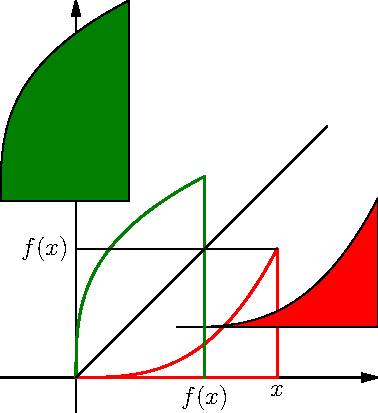
\includegraphics{./Cip11_1.pdf}
  % Cip11_1.pdf: 0x0 pixel, -2147483648dpi, 0.00x0.00 cm, bb=
  \caption{Exercice \theenumi \hspace{0.5cm }(Cip11)}
  \label{fig: Cip11_1}
\end{figure}
\begin{tiny}(Cip11)\end{tiny} Notons $I_1$ la première intégrale ($x$ en haut) et $I_2$ la deuxième ($f(x)$ en haut). Dans $I_2$, effectuons le changement de variable 
\begin{displaymath}
  t = f^{-1}(u)\rightsquigarrow u = f(t) \rightsquigarrow du = f'(t)dt 
\end{displaymath}
qui conduit à
\begin{displaymath}
  I_2 = \int_{0}^{x}tf'(t)dt
\end{displaymath}
puis une intégration par parties
\begin{displaymath}
  I_2 = \left[tf(t) \right]_{0}^{x}-\int_{0}^{x}f(t)dt = xf(x) - I_1
\end{displaymath}
On présente en figure \ref{fig: Cip11_1} une interprétation géométrique. La surface au dessous des graphes sont décalées pour faciliter la visualisation. Notons $S_1$ celle de droite attachée au graphe de $f$ et $S_2$ celle de gauche attachée au graphe de $f^{-1}$. L'aire est conservée par symétrie et la surface symétrique de $S_2$ par rapport à la bissectrice vient compléter $S_1$ pour former le rectangle.
